\subsection{Automaten}
Es wurde versucht Automaten sowohl möglichst nah an der theoretischen Vorgabe als auch möglichst effizient zu implementieren. Herausgekommen ist dabei folgende Grundimplementation:
\begin{figure}[h]
  \centering
  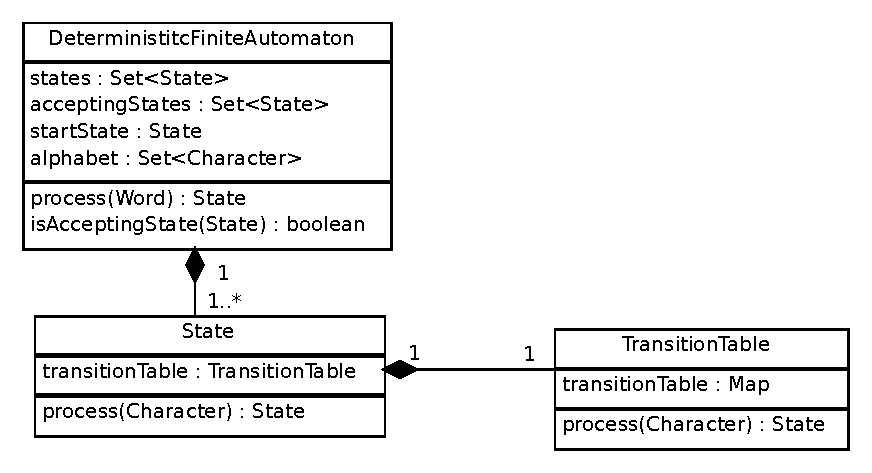
\includegraphics[width=0.5\textwidth]{images/dfa_classdiag_simple.pdf}
  \caption[DFA Klassendiagramm vereinfacht]{DFA Klassendiagramm vereinfacht}
  \label{fig:dfa_classdiag_simple}
\end{figure}

Das Quintupel ($Q$, $\Sigma$, $\delta$, $q0$, $F$) ist darin wie folgt abgebildet:

\begin{table}[h]
  \centering
  \begin{tabular}{ l | l }
    \hline
    $Q$ & Die Menge der Zustände wurde als Set von States implementiert.  \\
    \hline
    $\Sigma$ & Das Alphabet ist ein Array von Zeichen (Character). \\
    \hline
    $\delta$ & Die Übergangsfunktion $\delta$ wird als Map (Zeichen -> Zustand) 
    \\ & auf den einzelnen Zuständen abgebildet. Dies erlaubt uns eine
    \\ & einfache und effiziente Verarbeitung von Eingaben sowohl auf
    \\ & Zustands als auch auf Automaten Ebene. \\
    \hline
    $q0$ & Eine Referenz zum Startzustand $q0$ ist in der DFA Klasse hinterlegt. \\
    \hline
    $F$ & Die Menge der Akzeptierenden Zustände wird durch ein Set auf dem \\ & jeweiligen DFA Objekt representiert. \\
    \hline 
  \end{tabular}
  \caption[Implementation Automaten]{Implementation automaten}
\end{table}

Ein solcher Automat kann nun mithilfe seiner $process(Word)$ Funktion ein Wort (Eine Liste von Zeichen) verarbeiten indem er sich die Referenz des ersten Zustandes $startState$ holt und dann Zeichen für Zeichen jeweils mit $process(Character)$ die Referenz des nächsten Zustandes herausliest. Zurückgegeben wird schlussendlich derjenige Zustand der am Ende der verarbeiteten Zeichenkette erreicht wurde. Mithilfe der $isAcceptingState(State)$ Methode könnte man nun feststellen ob das Wort akzeptiert wird oder nicht. 

Zum besseren Verständnis folgend die Process Methode der DFA Klasse als Pseudocode:

\begin{lstlisting}[language=Python, caption={Process Methode der DFA Klasse}]
def process(word):
  state = startState
  for char in word:
    state = state.process(char)
  return state
\end{lstlisting}
